\documentclass[letterpaper, 12pt]{report}
\usepackage[margin=1in]{geometry}
\newcommand\R{\mathbb{R}}
\newcommand\Z{\mathbb{Z}}
\newcommand\pv[1]{\overrightarrow{#1}}
\newcommand\ihat{\hat i}
\newcommand\jhat{\hat j}
\newcommand\khat{\hat k}
\newcommand{\diagram}[2][0.5]{
	\begin{figure}[H]
		\centering
		\includegraphics[width=#1\textwidth]{#2}
	\end{figure}
	}

\usepackage{amsmath}
\usepackage{amssymb}
\usepackage{pgfplots} % plot math graphs
\usepackage{gensymb}
\usepackage{comment} % commenting functionality
\usepackage{tabularx} % better tabular env
\usepackage{pdfpages} % include pages from external pdf
\usepackage{float}
\usepackage{graphicx}
\graphicspath{ {./images/} }
\usepackage{amsthm}
\usepackage{hyperref} % hyperref should be the last package loaded

\DeclareMathOperator\cis{cis}

\theoremstyle{definition}
\newtheorem{thm}{Theorem}[section]
\newtheorem{cor}{Corollary}[thm]
\newtheorem{dfn}{Definition}[section]

\newcommand*\circled[1]{\tikz[baseline=(char.base)]{
	            \node[shape=circle,draw,inner sep=2pt] (char) {#1};}}

\pgfplotsset{every axis/.append style={
  axis x line=middle,    % put the x axis in the middle
  axis y line=middle,    % put the y axis in the middle
  axis line style={<->}, % arrows on the axis
  xlabel={$x$},          % default put x on x-axis
  ylabel={$y$},          % default put y on y-axis
}}

%\pgfplotsset{mystyle/.style={color=blue,no marks,line width=1pt,<->}} 
%\pgfplotsset{mystyle/.style={color=blue,<->}} 
\pgfplotsset{mystyle/.style={color=blue}} 

\tikzset{>=stealth}

\pgfplotsset{compat=1.17}
\usepgfplotslibrary{external}
\tikzexternalize[prefix=./cache/]

\title{Grade 11 Quad 4 Math Notes}
\author{Avaneesh Kulkarni}
\date{}

\setcounter{tocdepth}{2}
\numberwithin{equation}{section}

\begin{document}
\pagenumbering{gobble}
\maketitle
\tableofcontents
\newpage
\pagenumbering{arabic}

\chapter{Course 1 - MCR3U7}

\section{Review Unit}

\subsection{Quadratics Review}

\subsubsection*{Sum and Product of Roots of Quadratic}
For a quadratic equation, $ax^2 + bx + c = 0$ (where $a \neq 0$),
let $r_1, r_2$ be the roots. Then,

\begin{equation}\label{sumquad}
	r_1 + r_2 = -\frac{b}{a}
\end{equation}
and
\begin{equation}\label{prodquad}
	r_1 r_2 = \frac{c}{a}
\end{equation}

These can be proven by writing $r_1$ and $r_2$ in terms of a,b,c by using the quadratic formula.

Relation to equation:
\begin{align*}
	ax^2 + bx + c &= 0 \\ 
	\frac{ax^2 + bx + c}{a} &= 0 \\ 
	x^2 + \frac{b}{a}x + \frac{c}{a} &= 0 \\ 
	x^2 - \left( - \frac{b}{a} \right) x + \frac{c}{a} &= 0 \\ 
	x^2 - \mathrm{S} x + \mathrm{P} &= 0 
\end{align*}
where S is the sum of roots and P is the product of roots.

\subsubsection*{Sum and Product of Polynomial Roots}
In the general case, for a polynomial $P(x) = a_nx^n + a_{n-1}x^{n-1} + \dotsb + a_0 $,
\begin{equation}
	S = - \frac{a_{n-1}}{a_n}
\end{equation}
\begin{equation}
	P = (-1)^n \frac{a_0}{a_n}
\end{equation}
where S is the sum and P is the product of the roots.

These can be derived by comparing the coefficients of the following two forms of $P(x)$:
\begin{alignat*}{2}
	P(x) &= a_nx^n + a_{n-1}x^{n-1} + &&\dotsb + a_0 \\
	P(x) &= a(x-r_1)(x-r_2) &&\dotsm (x-r_n)
\end{alignat*}

\subsection{Complex Numbers Review}
For a complex number $z$,
\begin{itemize}
	\item Rectangular form: $z = a + bi$, where $a,b \in \mathbb{R} $
	\item Conjuagate: $z^* \textrm{ or } \bar{z} = a - bi$
	\item Modulus: $|z| = \sqrt{a^2 + b^2}$
\end{itemize}
Also, $z \times \bar{z} = {|z|}^2 = a^2 + b^2$

\subsection{Factor Theorem \& Remainder Theorem Review}
\paragraph{Notation:}
\begin{align*}
	P(x) \leftarrow &\textrm{ polynomial} \\
	D(x) \leftarrow &\textrm{ divisor} \\
	Q(x) \leftarrow &\textrm{ quotient} \\
	R(x) \leftarrow &\textrm{ remainder}
\end{align*}

\paragraph{Division statement (2 ways):}
\begin{equation}
	P(x) = D(x)Q(x) + R(x)
\end{equation}
\begin{center}
or
\end{center}
\begin{equation}
	\frac{P(x)}{D(x)} = Q(x) + \frac{R(x)}{D(x)}
\end{equation}

Note that in both forms, $D(x) \neq 0$.

\subsubsection*{Factor Theorem}
\begin{itemize}
	\item When $P(x)$ is divided by $x-b$ the remainder is $P(b)$.
If $P(b) = 0$, then $(x-b) | P(x)$.
	\item When $P(x)$ is divided by $ax-b$ the remainder is $P(\frac{b}{a})$.
If $P(\frac{b}{a}) = 0$, then $(ax-b) | P(x)$.
\end{itemize}

\subsection{Transformation of a Function Review}
\begin{samepage}
General form of a transformed function:
\begin{equation}
	f(x) = a\:[\:b\:(x-c)\:] + d
\end{equation}

\begin{tabular}{l l}
	$a > 0$ & no reflection \\
	$a < 0$ & reflection in x-axis \\
	$a > 1$ & vertical stretch by a factor of $a$  \\
	$0 < a < 1$ & vertical compression by a factor of $\frac{1}{a}$ \\
	$b < 0$ & reflection in y-axis \\
	$b > 1$ & horizontal compression by a factor of $b$  \\
	$0 < b < 1$ & horizontal stretch by a factor of $\frac{1}{b}$ \\
	$c > 0$ & horizontal translation $c$ units to the right \\
	$c < 0$ & horizontal translation $c$ units to the left \\
	$d > 0$ & vertical translation $d$ units up \\
	$d < 0$ & vertical translation $d$ units down 
\end{tabular}
\end{samepage}

\section{Rational Functions}
\begin{itemize}
	\item v.a. means vertical asymptote
	\item h.a. means horizontal asymptote
\end{itemize}
\subsection{Reciprocal of a Linear Function}
\begin{equation*}
	y = \frac{a}{kx-c}
\end{equation*}

\begin{tabular}{l l}
	v.a. & $x = \frac{c}{k}$ \\
	h.a. & $y=0$ \\
	y-int & $(0,\frac{a}{c})$
\end{tabular}

\begin{center}
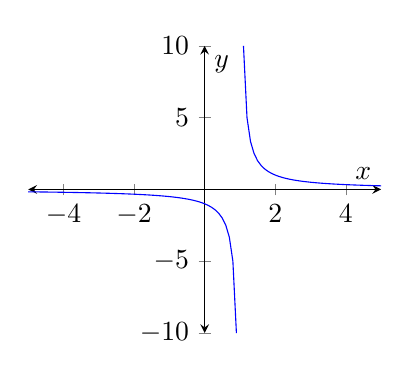
\begin{tikzpicture}
	\begin{axis}[width=0.5\textwidth]
		\addplot[mystyle,samples=101,unbounded coords=jump]{1/(x-1)};
\end{axis}
\end{tikzpicture}
\end{center}

\subsection{Reciprocal of a Quadratic}
\subsubsection{Two real roots}

\begin{equation*}
	y = \frac{a}{(x-r)(x-s)}
\end{equation*}

\begin{tabular}{l l}
	v.a.: & $x=r$ and $x=s$ \\
	h.a.: & $y=0$ \\
	local max at & $x=\frac{r+s}{2}$ (same as the parabola's vertex)
\end{tabular}

\bigskip 

\begin{center}
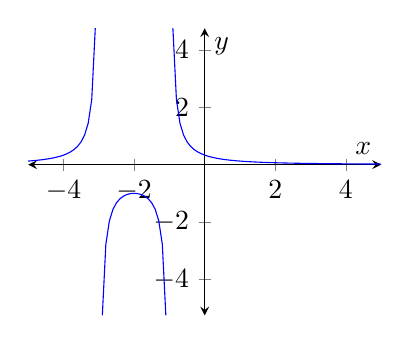
\begin{tikzpicture}
	\begin{axis}[width=0.5\textwidth]
		\addplot[mystyle,samples=101,unbounded coords=jump]{1/(x^2+4*x+3)};
\end{axis}
\end{tikzpicture}
\end{center}

\subsubsection{One real root}
\begin{equation*}
	y = \frac{a}{(x-r)^2}
\end{equation*}
\begin{tabular}{l l}
	v.a.: & $x=r$ \\
	h.a.: & $y=0$ 
\end{tabular}

\begin{center}
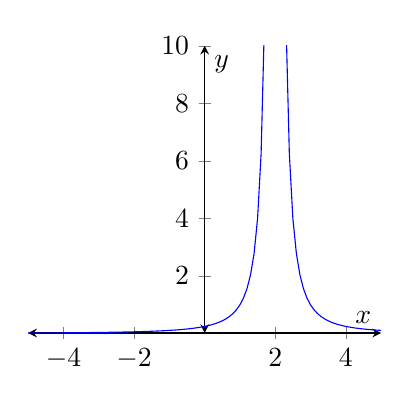
\begin{tikzpicture}
	\begin{axis}[
			ymax=10,
			width=0.5\textwidth
		]
		\addplot[mystyle,samples=101,unbounded coords=jump]{1/((x-2)^2)};
\end{axis}
\end{tikzpicture}
\end{center}

\subsubsection{No real roots}
\begin{equation*}
	y = \frac{a}{(x-r)^2 + b}
\end{equation*}
\begin{tabular}{l l}
	h.a.: & $y=0$ \\
	local max at & $x=\frac{r+s}{2}$ (same as the parabola's vertex)
\end{tabular}

\begin{center}
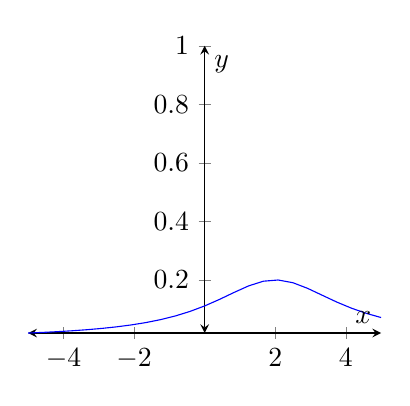
\begin{tikzpicture}
	\begin{axis}[
			ymax=1,
			xmin=-5, xmax=5,
			width=0.5\textwidth
		]
		\addplot[mystyle]{1/((x-2)^2+5)};
\end{axis}
\end{tikzpicture}
\end{center}

\subsection{Linear divided by Linear}
\begin{equation*}
	y = \frac{ax+b}{cx+d}
\end{equation*}
\begin{tabular}{l l}
	v.a.: & $x=-\frac{d}{c}$ \\
	h.a.: & $y=\frac{a}{c}$ \\
	&\\
	y-int: & $\left(0,\frac{b}{d}\right)$ \\
	&\\
	x-int: & $\left(-\frac{b}{a}, 0\right)$ 
\end{tabular}

\begin{center}
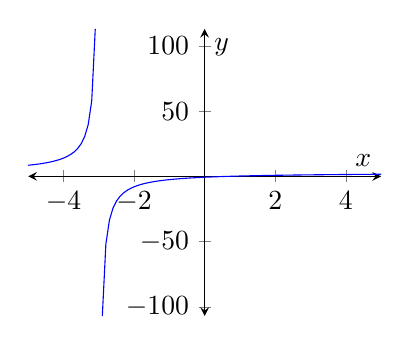
\begin{tikzpicture}
	\begin{axis}[
			width=0.5\textwidth
		]
		\addplot[mystyle,samples=101,unbounded coords=jump]{(3*x-2)/(x+3)};
\end{axis}
\end{tikzpicture}
\end{center}

Remember to label h.a. and v.a. when graphing.

Also label x-axis and y-axis.
\subsection{General Rational Functions}
Given two ploynomial functions, $P(x)$ of degree p, and $Q(x)$ of degree q, the function $\frac{P(x)}{Q(x)}$:
\begin{itemize}
	\item has a horizontal asymptote $y=0$ if $q>p$
	\item has a horizontal asymptote $y=k$ if $q=p$
		\begin{itemize}
			\item where k is found by dividing the leading cofficients
		\end{itemize}
	\item has an oblique asymptote if $p>q$ and that asymptote has order $p-q$.
\end{itemize}
\subsection{Rational Equations and Inequalities}
\subsubsection*{Equations}
Method:
\begin{enumerate}
	\item Note the restrictions on x (values that make the denominator are 0. \label{one}
	\item Make both LHS and RHS into 1 fraction each.
	\item Cross-multiply, expand, simplify, and solve.
	\item Check that the solutions are valid from step \ref{one}.
\end{enumerate}

\subsubsection*{Inequalities}
Method:
\begin{enumerate}
	\item Bring all the terms to the left side, forming a rational function.
	\item Use a factor table to find where the rational function is positive or negative.
	\item Account for vertical asymptotes. The LHS can be zero at x-intercepts but not at vertical asymptotes.
\end{enumerate}

\section{Absolute Value Function}
\begin{center}
\begin{tikzpicture}
	\begin{axis}[width=7cm]
	\addplot[mystyle]{abs(x)};
\end{axis}
\end{tikzpicture}
\end{center}
%Domain: $\{ x \:|\: x \in \R \}$
%Range: $\{ y \:|\: y \in \R, y \ge 0\}$

Note that:
\begin{equation} \label{absprop}
	|x| \;= \sqrt{x^2}
\end{equation}

\subsubsection*{Properties of the Absolute Value Function}
\begin{itemize}
	\item $\displaystyle |ab| = |a| \times |b|$
	\item $\displaystyle \left|\frac{a}{b}\right| = \frac{|a|}{|b|}$ (if $b \neq 0$)
\end{itemize}

\subsection{$|f(x)|$ and $f(|x|)$}
For $|f(x)|$, simply fold the parts of $f(x)$ that are below the x-axis over the x-axis. Note that this may create cusps in the graph.

\vspace{1em}

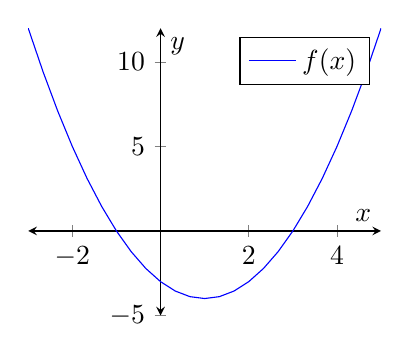
\begin{tikzpicture}
	\begin{axis}[
			width=0.5\textwidth,
			ymin=-5,
			legend pos = north east
		]
		\addplot[mystyle,domain=-3:5]
		{(x+1)*(x-3)};
		\addlegendentry{$f(x)$}
\end{axis}
\end{tikzpicture}
\hskip 30pt
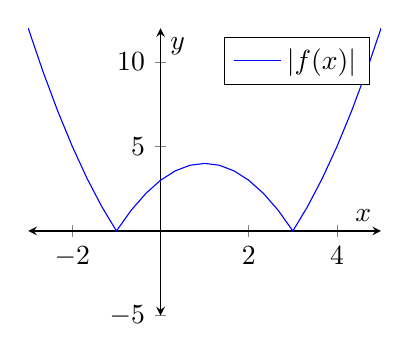
\begin{tikzpicture}
	\begin{axis}[
			width=0.5\textwidth,
			ymin=-5,
			legend pos = north east
		]
		\addplot[mystyle,domain=-3:5]
		{abs((x+1)*(x-3))};
		\addlegendentry{$|f(x)|$}
\end{axis}
\end{tikzpicture}

For $f(|x|)$, erase the part of the graph to the left of the y-axis, and reflect the remaining part across the y-axis. For example,

\vspace{1em}

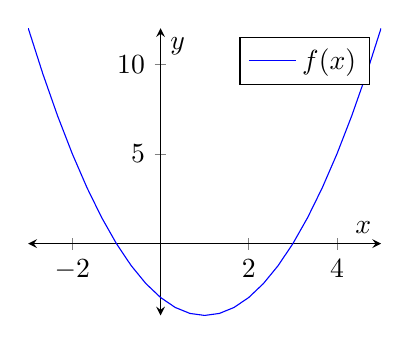
\begin{tikzpicture}
	\begin{axis}[
			width=0.5\textwidth,
			legend pos = north east
		]
		\addplot[mystyle,domain=-3:5]
		{(x+1)*(x-3)};
		\addlegendentry{$f(x)$}
\end{axis}
\end{tikzpicture}
\hskip 30pt
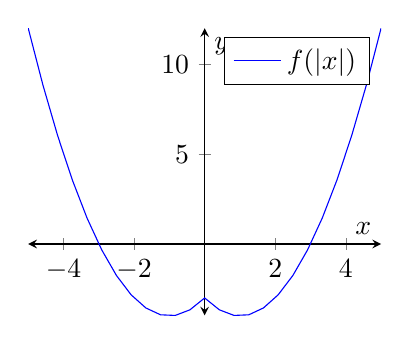
\begin{tikzpicture}
	\begin{axis}[
			width=0.5\textwidth,
			legend pos = north east
		]
		\addplot[mystyle]
		{(abs(x)+1)*(abs(x)-3)};
		\addlegendentry{$f(|x|)$}
\end{axis}
\end{tikzpicture}

\subsection{Absolute Value Equations and Inequalities}

\paragraph{Equations}

Examine each interval seperately (use cases). For example, if the equation is

\begin{equation*}
	|3x-4| + 4x^2 - 2 = |5x+1|
\end{equation*}

\medskip

the cases would be $x \in (-\infty, -\frac{1}{5}), [-\frac{1}{5}, \frac{4}{3}), [\frac{4}{3}, \infty)$. Remember to include the boundary values of x only once ($-\frac{1}{5}$ and $\frac{4}{3}$).

Each term in absolute value brackets will be positive or negative depending on the interval.

Remember to reject values of $x$ which fall outside the domain being considered in that case.

\bigskip

Note: Another method is to square both sides to remove absolute values by using this identity \eqref{absprop}. However, that method may introduce extraneous solutions because squaring is a non-reversible operation. If using that method, remember to verify all solutions.

\paragraph{Inequalities}

For simple inequalities, this rule may suffice

\medskip

\begin{tabular}{l l}
	If $|f(x)| < a$, &where $a>0$, then $-a<x<a$ \\
	If $|f(x)| > a$, &where $a>0$, then $x<-a$ or $x>a$
\end{tabular}

\medskip

For more complex ones, examine each interval seperately like you do when solving absolute value equalities. Remember to verify that the solution is inside the domain of that case. If the solution partially overlaps with the domain, take the intersection of the two intervals.

\section{Inverse and Composite Functions}

$f \circ g(x)$ is read as "f compose g of x". It is synonymous to $f(g(x))$.

\bigskip \noindent
Note that $f \circ g(x) \ne g \circ f(x)$. (composition is not always commutative)

\bigskip \noindent
But $f \circ f^{-1} = f^{-1} \circ f(x) = x$.

\bigskip \noindent
Self inverse function: $f(x) = f^{-1}(x)$.

\bigskip \noindent
Given $f(x)$, to find the intersection of $f(x)$ and $f^{-1}(x)$ without solving for $f^{-1}(x)$, you simply find the intersection of $f(x)$ and $y=x$. This works because $f^{-1}(x)$ is a reflection of $f(x)$ across the line $y=x$.

\subsection{Techniques to Solve Function Composition Problems}

There are 2 common types of function composition problems:

\begin{enumerate}
	\item Given $(f \circ g)(x) = \dotso$ and $f(x)= \dotso$, find $g(x)$
	\item Given $(f \circ g)(x) = \dotso$ and $g(x)= \dotso$, find $f(x)$
\end{enumerate}

If you are given the outer function (type 1), plug in $g(x)$ into $(f \circ g)(x)$, and solve for $g(x)$.

If you are given the inner function (type 2), first find $g^{-1}(x)$ and then plug in $g^{-1}(x)$ into $(f \circ g)(x)$. This will give,

\begin{equation*}
	f(g(g^{-1}(x))) = g^{-1}(x)^2 + 4g^{-1}(x) + \dotsb = f(x)
\end{equation*}

and you will have found an expression for $f(x)$.

\section{Reciprocal and Square of a Function}
Think of squaring and reciprocating $f(x)$ as applying a transformation onto $f(x)$.

\subsection{Square of a function}
Given $f(x)$, graph $[f(x)]^2$.
\begin{enumerate}
	\item Invariant points have $y=0,1$. Also, points which have a y-coordinate of -1 are reflected across the x-axis.
\item The horizontal asymptote is squared.
\item For, $f(x)>0$ it seems like a vertical stretch. For $f(x)<0$, reflect across y-axis, then stretch. 
\item Sharp points in the graph of $f(x)$, such as those in $y=|x|$, may become cusps.
\end{enumerate}

The horizontal asymptote is transformed, but the vertical asymptote remains the same.

If $f(x)$ is approximately a line at its x-intercept, $[f(x)]^2$ has a curve which touches the x-axis at that point. This is because the square of a linear expression is a quadratic (parabola).

In general, any part of $f(x)$ that is a line becomes a parabola.

\subsection{Reciprocal of a function}
\begin{enumerate}
	\item Invariant points have $y=-1,1$.
	\item Vertical asymptotes become x-intercepts.
	\item x-intercepts become vertical asymptotes.
	\item Horizontal asymptotes are reciprocated.
	\item If $f(x)>0$, $\frac{1}{f(x)}>0$
	\item If $f(x)<0$, $\frac{1}{f(x)}<0$
	\item If $f(x)>1$, $\frac{1}{f(x)}<1$
	\item If $f(x)<1$, $\frac{1}{f(x)}>1$
\end{enumerate}

Examine each branch individually and reason out how the reciprocal would look like.

\section{Exponential and Logarithmic Functions}
\subsection*{Exponent terminology}
\begin{equation*}
	\sqrt[n]{x}
\end{equation*}
\begin{samepage}
\begin{center}
\begin{tabular}{l l}
	$n$ & is called the index \\
	$x$ & is called the radicand 
\end{tabular}
\end{center}
\end{samepage}
\begin{samepage}
Also in the exponential form:
\begin{equation*}
	a^{\textstyle\frac{b}{c}}
\end{equation*}
\begin{center}
\begin{tabular}{l l}
	$b$ & is the exponent \\
	$c$ & is the index 
\end{tabular}
\end{center}
\end{samepage}

\subsection{Exponential Functions}
\begin{equation*}
	f(x) = a^x
\end{equation*}
Where $a > 0$, $a \ne 1$.
\subsection{Logarithmic Functions}
\begin{equation*}
	f(x) = \log_b x
\end{equation*}
Where $x > 0$, $b > 0$, $b \ne 1$.

\bigskip \noindent
$y = \log_a x$ is the inverse of $y = a^x$.
\paragraph{Power Law}
\begin{equation}
	\log_{b^m}(x^n) = \frac{n}{m} \times \log_b x
\end{equation}

\subsection{Expontential Growth and Decay}
\paragraph{Growth}
\begin{equation}
	N(t) = N_0 (2)^{\textstyle\frac{t}{h}}
\end{equation}
\paragraph{Decay}
\begin{align}
	N(t) &= N_0 \left(\frac{1}{2}\right)^{\textstyle\frac{t}{h}} \label{1} \\
			 &= N_0 (2)^{-\textstyle\frac{t}{h}} \label{2}
\end{align}

\begin{tabular}{l l}
	$N(t)$ & is final amount \\
	$N_0$ & is initial amount \\
	$t$ & is time \\
	$h$ & is half-life (same units as $t$)
\end{tabular}

\bigskip \noindent
Both \eqref{1} and \eqref{2} can be used to solve problems.

\paragraph{General Form}
\begin{equation}
	N(t) = N_0 e^{\textstyle\frac{k}{t}}
\end{equation}

where $k$ is the exponential growth/decay constant of the specific situation. $k$ can be calculated if you are given the half-life or doubling time (or even the time it takes to reach some fraction/multiple of the original amount.

\bigskip \noindent
\begin{tabular}{l l}
	If $k > 0$ & it's exponential growth \\
	If $k < 0$ & it's exponential decay
\end{tabular}

\subsection{Compound Interest} \label{cmpint}
\paragraph{Non-continuous}
\begin{samepage}
\begin{equation}
	A = P {\left( 1 + \frac{r}{n} \right)} ^ {nt}
\end{equation}

\begin{tabular}{l l}
	$A$ & is the final amount \\
	$P$ & is the initial amount \\
	$r$ & is the interest rate (in decimal form) \\
	$n$ & is the compounding period \\
	$t$ & is the time (years)
\end{tabular}
\end{samepage}

\bigskip \noindent
$n$ refers to how frequently the interest is paid. For example:
\begin{center}
\begin{tabular}{l l}
	monthly & means $n=12$ \\
	quarterly& means $n=4$ \\
	semi-annually & means $n=2$ \\
	annually & means $n=1$
\end{tabular}
\end{center}

\paragraph{Continous Compounding}
\begin{equation} \label{cont}
	A = P e^{rt}
\end{equation}

Use \eqref{cont} when the interest compounds continually.

\section{Sequences and Series}

\subsection{Sequences}
A sequence is a function whose domain is a subset of the set of natural numbers ($\mathbb{N}$). The values in the range are called the terms of the sequence.

\begin{center}
Ex. $20, 15, 10, 5, \dotso , -30$

\bigskip

\begin{tabular}{l | l}
	x & y \\ \hline 
	1 & 20 \\
	2 & 15 \\
	3 & 10 \\
	4 & 10 
\end{tabular}
\end{center}

\subsubsection{Arithmetic Sequences}

A sequence is arithmetic if the difference between the terms is constant. The general term of an arithmetic sequence is

\begin{equation}
	t_n = a + (n-1) d
\end{equation}

\begin{tabular}{l l l}
	where & $a$ &is the first term \\
	& $d$ &is the common difference ($d = t_n - t_{n-1}$) \\
	& $n$ &is the number of terms 
\end{tabular}

\subsubsection{Geometric Sequences}

A sequence is geometric if the \emph{ratio} between the terms is constant. The general term of a geometric sequence is

\begin{equation}
	t_n = ar^{n-1} 
\end{equation}

\begin{tabular}{l l l}
	where & $a$ &is the first term \\
	& $r$ &is the common ratio $\left(r = \frac{t_n}{t_{n-1}} \right)$ \\
	& $n$ &is the number of terms 
\end{tabular}

\subsubsection{Arithmetic Means}
If a question says ``insert $n$ arithmetic means between $a$ and $b$", where n,a,b are given, you need to find $n$ numbers between $a$ and $b$ which form an arithmetic sequence along with $a$ and $b$.

\subsubsection{Geometric Means}
If a question says ``insert $n$ geometric means between $a$ and $b$", where n,a,b are given, you need to find $n$ numbers between $a$ and $b$ which form a geometric sequence along with $a$ and $b$.

\subsubsection{Simple Interest}
Unlike compound interest (\ref{cmpint}), \emph{simple} interest means you only receive interest on the original amount. For example, a simple interest of 6\% per annum on an investment of \$200, means the amount will be

\begin{center}
	\$200, \$212, \$224, \$236, \dotso
\end{center}
which makes it an arithmetic series.

\subsection{Series}
A series is the sum of the terms of a sequence.
Given a sequence $t_1, t_2, t_2, \dotsc, t_n$,
$S_n$ denotes the sum of the first $n$ terms.
This is called a partial sum.

\subsubsection{Arithmetic Series}

\begin{align}
	S_n & = \frac{n}{2} (a + t_n) \label{arithseries1} \\
	S_n & = \frac{n}{2} (2a + (n-1) d ) \label{arithseries2}
\end{align}

\noindent
Proof.

\begin{alignat*}{6}
	S_n & = t_1 && + t_2     && + t_3     && + \dotsb && + t_{n-1} && + t_n \\
	S_n & = t_n && + t_{n-1} && + t_{n-2} && + \dotsb && + t_2     && + t_1
\end{alignat*}
Writing both of these in terms of $a$ and $d$ gives
\begin{alignat*}{6}
	  S_n & = a        && + a+d      && + \dotsb && + a+(n-2)d && + a  + (n-1)d \\
		S_n & = a+(n-1)d && + a+(n-2)d && + \dotsb && + a+d      && + a 
\end{alignat*}
Adding the two,
\begin{equation}
	2 S_n = 2a+(n-1)d + 2a+(n-1)d + \dotsb + 2a+(n-1)d + 2a + (n-1)d
\end{equation}
\begin{align*}
	2 S_n & = n(2a + (n-1)d) \\
	S_n & = \frac{n}{2}(2a + (n-1)d)
\end{align*}
which gives \eqref{arithseries2}. To get \eqref{arithseries1} we can continue,
\begin{align*}
	S_n & = \frac{n}{2}(a + (a + (n-1)d)) \\
	S_n & = \frac{n}{2}(a + t_n) 
\end{align*}

\subsubsection{Geometric Series}

\begin{alignat}{2}
	S_n & = && \frac{a(1-r^n)}{1-r}, \qquad r \ne 1 \label{geoseries1} \\
	S_n & = && \frac{a(r^n - 1)}{r-1}, \qquad r \ne 1 \label{geoseries2} 
\end{alignat}

Proof.
\begin{alignat*}{2}
	S_n & = a + ar + ar^2 + \dotsb + ar^{n-2} + ar^{n-1} \\
	r S_n & = ar + ar^2 + \dotsb + ar^{n-2} + ar^{n-1} + ar^n \\
	S_n - rS_n & = a - ar^n \\
	S_n(1-r) & = a(1-r^n) \\
	S_n & = \frac{a(1-r^n)}{1-r}
\end{alignat*}
which gives \eqref{geoseries1}.

\bigskip
\noindent
Sum of infinite geometric series:
\begin{equation}
	 S_\infty = \frac{a}{1-r}
\end{equation}


\noindent
A useful equation to solve problems is

\begin{equation} \label{extra}
	t_n = S_n - S_{n-1}
\end{equation}

\eqref{extra} is useful when you are given an expression for $S_n$ and asked to find one of the terms of $t$.

\subsubsection{Sigma notation}
Properties:

\begin{align}
	&\sum_{i=1}^n c = cn \\
	&\sum_{i=1}^n c \,t_i = c \sum_{i=1}^n t_i \\
	&\sum_{i=1}^n (a_i \pm b_i) = \sum_{i=1}^n a_i \pm \sum_{i=1}^n b_i \\
	&\sum_{i=1}^n t_i = \sum_{i=1}^c t_i + \sum_{i=c+1}^n t_i , \quad 1 < c < n 
\end{align}

\section{Trig Review}
\begin{equation*}
	\sin^{-1} \ne csc
\end{equation*}

Because $\sin^{-1}$ denotes the inverse function of $\sin$, which is $\arcsin$. This is similar to how $f^{-1}(x)$ denotes the inverse function of $f$.

But note that $\sin^2(x) = [ \sin(x) ]^2$, or $\sin^3(x) = [\sin(x)]^3$, etc.

\subsection{Terminology}
\paragraph{Standard form} An angle in standard form has one arm on the positive $x$-axis, called the initial arm, and the other arm anywhere else, called the terminal arm.
\paragraph{Principal angle} The counter clockwise angle between the initial and terminal arm of an angle in standard position.
\paragraph{Co-terminal angles}
are angles whose terminal arms have the same standard position. If $\alpha$ and $\theta$ are co-terminal angles,
\begin{equation}
	\alpha - \theta = k \times 360 \degree \quad \textrm{ where } k \in \mathbb{Z}
\end{equation}
or in other words
\begin{equation}
	\alpha = k \times 360 \degree + \theta \quad \textrm{ where } k \in \mathbb{Z}
\end{equation}
So to find a co-terminal angle of $\theta$ you can simply add or subtract multiples of $360 \degree$.
\paragraph{Related Acute Angle (RAA)} a.k.a. \textbf{Reference Angle (RA)} is the positive acute angle between the terminal arm and $x$-axis of an angle in standard position.
\paragraph{Angle of Elevation/Depression}
in word problems, the angle of elevation or depression is the angle made from the horizontal to the line of sight.

\subsection{Method to Evaluate a Trig Ratio}
First find the RAA of $\theta$. Let's call it $\alpha$. Then calculate $\sin\alpha$. Then use the CAST rule to determine the sign of $\sin\theta$ and apply it to $\sin\alpha$.

\subsection{Circle Stuff}
\subsubsection{Radians}
\begin{equation}
	1 \textrm{ rad } = \frac{180 \degree}{\pi}
\end{equation}
\begin{equation}
	1 \degree = \frac{\pi}{180 \degree} \textrm{ radians}
\end{equation}

\subsubsection{Sectors and Segments}
Arc length, a
\begin{equation} \label{arc}
	a = r \theta
\end{equation}

\bigskip
\noindent
Area of a sector, A
\begin{equation} \label{sector}
	A = \frac{r^2}{2} \theta
\end{equation}

\bigskip
\noindent
Area of a segment, A
\begin{equation} \label{segment}
	A = \frac{r^2}{2} (\theta - \sin \theta)
\end{equation}

\bigskip
\noindent
Note that $\theta$ is in radians.

\subsection{Compass Bearings}
\paragraph{Compass Bearing}
an angle measured from a specified direction. For example, South $30\degree$ East (or S30\degree E) means an angle $30\degree$ East from the South direction.

\paragraph{True Bearing}
like a compass bearing but always measured from North. For example, the true bearing 150\degree T is the same as the compass bearing S30\degree E. Also, if the angle is less than $100 \degree$, prepend with a zero. For example: 040\degree T.

\subsection{Graphing Trig Functions}
General form
\begin{equation}
	y = A \sin [k(x-a)] + c
\end{equation}
\medskip
\begin{tabular}{l l}
	A & is amplitude (vertical stretch) $\left( \frac{\mathrm{max} - \mathrm{min}}{2} \right)$ \\
	$y=c$ & is the equation of the sinusoidal axis (the midline) $\left(\frac{\mathrm{max}+\mathrm{min}}{2}\right)$ \\
	a & is phase shift \\
	$\frac{2\pi}{k}$ & is the period
\end{tabular}

\noindent
Important Increment (II): $\frac{\mathrm{period}}{4}$

\bigskip
\noindent
\begin{tabularx}{\textwidth}{ X | X | X | X | X }
	Num of II & 1 & 2 & 3 & 4 \\ \hline
	sin & axis & max & axis & min \\ \hline
	cos & max & axis & min & axis
\end{tabularx}

\paragraph{Scaling Increments (SI)}
When graphing, the smallest tick on the $x$-axis should divide the phase shift and II. Let's call the smallest tick length the Scaling Increment, or SI.
The SI is used as the smallest tick mark when graphing.
\begin{equation*}
	\textrm{An easy way to find the SI for: }\left( \frac{\pi}{a}, \frac{\pi}{b} \right) \textrm{ is } \frac{\pi}{\mathrm{lcm}(a,b)}
\end{equation*}

\subsection{Steps to Graph}
\begin{enumerate}
	\item Find $\mathrm{max}=c+a$ and $\mathrm{min}=c-a$
	\item Determine $\mathrm{period}=\frac{2\pi}{k}$
	\item Calculate $\mathrm{II}=\frac{\mathrm{period}}{4}$
	\item Calculate Scaling Increment
	\item Graph using the pattern for $\sin$ or $\cos$. Remember to account for reflections and phase shift.
\end{enumerate}

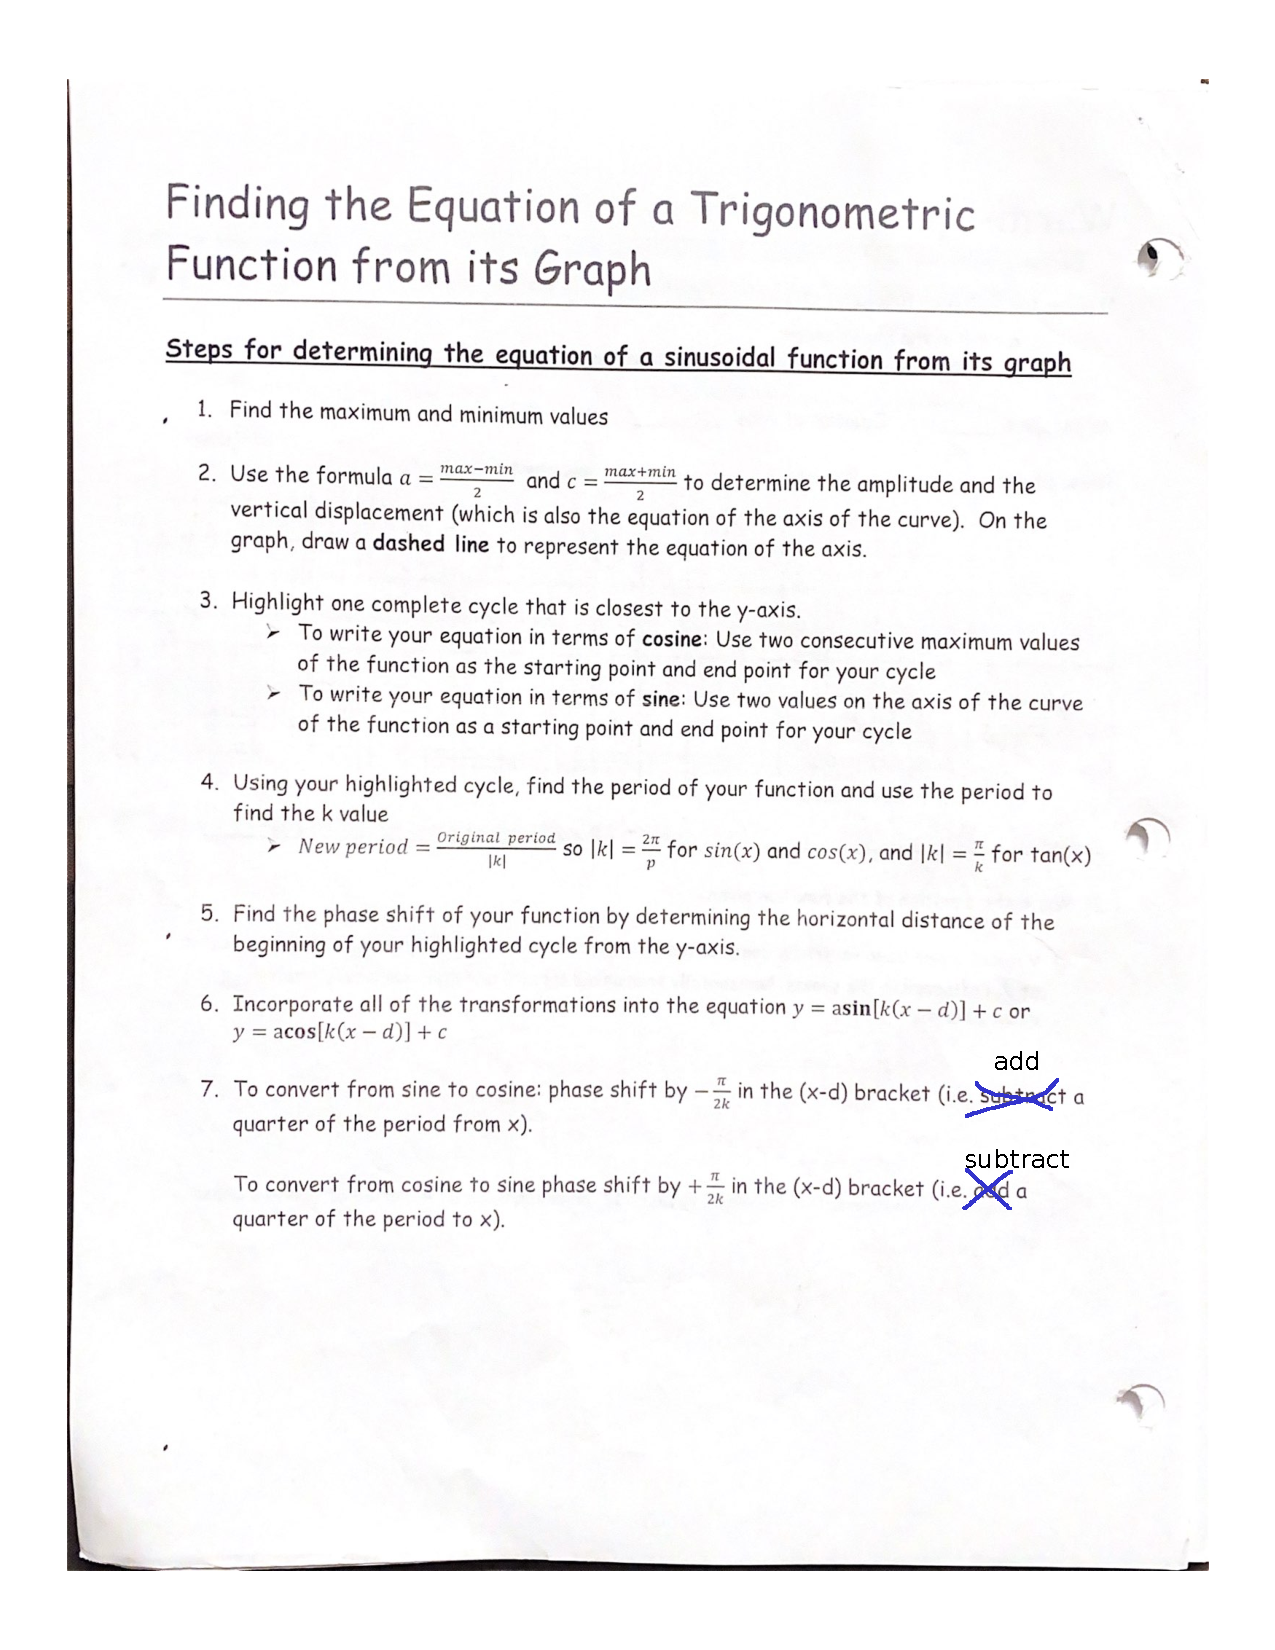
\includepdf[pagecommand={}]{images/finding-equation-of-sin-function.pdf}

\section{General Solutions to Trig Problems}
Solutions come in multiples of the period, so the final answer would look like:
\begin{equation*}
	\theta = \frac{7\pi}{6} + k \pi \quad \textrm{or} \quad \theta = \frac{\pi}{6} + k \pi, \qquad k \in \Z
\end{equation*}

If a domain is given, find all the solutions in the domain, otherwise, write down the general solution. 

\subsection{Inverse Trig Functions}

\paragraph{$\sin ^{-1} x$}
\begin{tabular}{l l}
	Domain: & $-1 \le x \le 1$\\
	Range: & $-\frac{\pi}{2} \le y \le \frac{\pi}{2}$ 
\end{tabular}

\paragraph{$\cos ^{-1} x$}
\begin{tabular}{l l}
	Domain: & $-1 \le x \le 1$ \\
	Range: & $0 \le y \le \pi$ 
\end{tabular}

\paragraph{$\tan ^{-1} x$}
\begin{tabular}{l l}
	Domain: & $-1 \le x \le 1$ \\
	Range: & $-\frac{\pi}{2} \le y \le \frac{\pi}{2}$ 
\end{tabular}

\bigskip

The following equations hold only when $x$ is in the range of $\sin^{-1}$ or $\cos^{-1}$.
\begin{alignat*}{2}
	\sin ^ {-1} ( \sin x ) &= x  \\
	\cos ^ {-1} ( \cos x ) &= x  \\
	\tan ^ {-1} ( \tan x ) &= x  
\end{alignat*}
Note that if the inverse function is on the inside it always equals x. For example $\sin( \sin^{-1} x )$ for all $x$ such that $-1 \le x \le 1$.

\subsection{Identities}

These are also called Pythagorean Identities
\begin{alignat}{2}
	1 + \tan ^2 x &= \sec ^ 2x \\
	1 + \cot ^2 x &= \csc ^2 x
\end{alignat}

\begin{comment}
\section{Test Topics}
\subsection{Test 1}
\subsection{Test 2}
\begin{itemize}
	\item Graph \& Features:
		\begin{itemize}
			\item $\displaystyle \frac{\mathrm{constant}}{\mathrm{linear}}$, $\displaystyle \frac{\mathrm{constant}}{\mathrm{quadratic}}$
			\item $\displaystyle \frac{\mathrm{linear}}{\mathrm{linear}}$, others (discontinuity, oblique vs h.a.)
		\end{itemize}
	\item Solving Rational Equations and Inequalities
	\item Square and Reciprocal of a Function
	\item Abs Value Eqn and Inequalities
	\item IB Questions
\end{itemize}
\end{comment}

\section{Complex Numbers}
\paragraph{Cartesian (or Rectangular Form)}
\begin{equation*}
	z = a + bi
\end{equation*}
\paragraph{Polar form}
\begin{equation*}
	z = r \cis ( \theta + 2 \pi k )
\end{equation*}
\begin{tabular}[]{l l}
	r & is the modulus $\left( r = \sqrt{a^2+b^2} \right)$ \\
	$\theta$ & is the argument
\end{tabular}

\subsection{Adding and Subtracting in Polar Form}
Polar form gives you nothing special for adding/subtracting. Convert to cartesian form then add/subtract.

\subsection{Multiplying in Polar Form}
\begin{alignat*}{2}
	( r_1 \cis \theta_1 ) ( r_2 \cis \theta_2 ) &= [ r_1 ( \cos \theta_1 + i \sin \theta_1 ) ] [ r_2 ( \cos \theta_2 + i \sin \theta_2 ) ] \\
	&= r_1r_2 [ \cos\theta_1\cos\theta_2 - \sin\theta_1\sin\theta_2 + i ( \sin\theta_1\cos\theta_2 + \sin\theta_2\cos\theta_1)] \\
	&= r_1r_2 [ \cos ( \theta_1 + \theta_2 ) + i \sin ( \theta_1 + \theta_2 ) ] \\
	&= r_1r_2 \cis ( \theta_1 + \theta_2 )
\end{alignat*}

When mulitplying complex numbers in polar form, \emph{magnitudes multiply and angles add}.

\subsection{Conjugate}
If $z = a + bi = r \cis \theta$, then the conjugate, $\overline{z}$ or $z^*$ is:

\begin{equation}
	z^* = r \cis ( - \theta )
\end{equation}
You can see this graphically.

\medskip
\noindent
Recall:
\begin{alignat*}{2}{}
	z z^* &= (a+bi)(a-bi) \\
	      &= a^2 + b^2 \\
				&= | z | ^2
\end{alignat*}
In polar form, this becomes,
\begin{alignat*}{2}{}
	z z^* &= (r\cis \theta ) ( r \cis ( - \theta	) ) \\
			 &= r^2 \cis ( \theta - \theta ) \\
			 &= r^2 ( \cos 0 + i \sin 0 ) \\
			 &= r^2 \\
			 &= | z | ^2
\end{alignat*}
In the above equations, you can skip a step if you see that since the argument $\theta - \theta = 0$, the number lies on the Real-axis.

\subsection{Division}
Recall: to divide complex numbers, we multiply the numerator and denominator by the conjugate.

\begin{alignat*}{2}{}
	\frac{r_1 \cis \theta_1}{r_2 \cis \theta_2} = \frac{z_1}{z_2} &= \frac{z_1 \overline{z}_2}{z_2\overline{z}_2} \\
	&= \frac{(r_1\cis\theta_1)(r_2\cis(-\theta_2))}{r^2} \\
	&= \frac{r_1}{r_2}\cis(\theta_1-\theta_2
\end{alignat*}

\chapter{Course 2 - MDM4U7}

\section{Vectors}
\subsection{Basic Definitions}
Vectors have:
\begin{itemize}
	\item initial point (tail)
	\item terminal point (tip)
\end{itemize}
\diagram[0.6]{vector}
The \textbf{magnitude} of a vector $\vec u$ is denoted by $| \vec u |$.

\bigskip \noindent
\textbf{Free vector}: a vector whose position is not fixed.

\subsubsection{Vector Equality (definition)}
Two vector are equal if and only if:
\begin{itemize}
	\item they have the same magnitude
	\item they have the same direction	
\end{itemize}
we write $\vec u = \vec v$ if they are equal.

\subsubsection{Vector Addition (definition)}
Place the tail of $\vec v$ on the tip of $\vec u$. $\vec u + \vec v$ is defined as the vector from the tail of $\vec u$ to the tip of $\vec v$.
\diagram{vector-add}

Or, you can use the parallelogram law.

\diagram{vector-parallelogram}

$\vec u + \vec v$ is called the \textbf{sum} or \textbf{resultant} of $\vec u$ and $\vec v$.

\subsubsection{Angles between Vectors}
The angle between two vectors is the angle formed when the vectors are placed \emph{tail to tail}.
\diagram{vector-angle}

\subsubsection{Opposite}
The \emph{opposite} of $\vec u$ is a vector with the same magnitude but exactly opposite direction. The opposite of $\vec u$ is denoted by $- \vec u$. The sum of a vector and its opposite is a vector with zero magnitude. This vector is called a \emph{zero vector} or $\vec 0$.

\begin{equation}
	\vec u + ( - \vec u ) = \vec 0
\end{equation}
A zero vector has indeterminate direction and magnitude 0.

\subsubsection{Vector Subtraction}
Vector subtraction is defined as ``adding the opposite''.
\begin{equation}
	\vec u - \vec v = \vec u + ( - \vec v), \quad \textrm{ by definition}
\end{equation}
It can also be illustrated as:
\diagram[0.4]{vector-subtract}

\subsubsection{Unit Vector}
A unit vector is a vector with magnitude 1.
A unit vector in the direction of any vector $\vec u$ can be found by dividing $\vec u$ by its magnitude.
\begin{equation}
	\hat u = \frac{\vec u}{|\vec u|}
\end{equation}
where $\hat u$ is a unit vector.

\subsubsection{Properties of Vector Addition}
\begin{gather}
	\vec u + \vec v = \vec v + \vec u \\
	\vec u - \vec v = \vec u + ( - \vec v ) \\
	\vec u + ( - \vec u ) = \vec 0 \\
	\vec u + ( \vec v + \vec w ) = ( \vec u + \vec v ) + \vec w
\end{gather}

\subsubsection{Multiplying Vectors by Scalars}
For vector $\vec u$ and real number $c$, the \textbf{scalar multiple of $\vec u$ by $c$} is a vector with the following characteristics:

\begin{tabular}{l l}
	magnitude: & $|c| \times |\vec u|$ \\
	direction: & if $c > 0$, same as that of $\vec u$ \\
	           & if $c < 0$, opposite to that of $\vec u$
\end{tabular}

This vector is denoted by $c \vec u$.

\subsubsection{Properties of Scalar Multiplication}
For vectors $\vec u$ and $\vec v$, and scalars $a$ and $b$,

\begin{gather}
	a ( \vec u + \vec v ) = a \vec u + a \vec v \\
	( a + b ) \vec u = a \vec u + b \vec u \\
	(ab) \vec u = a (b\vec u)
\end{gather}

\subsection{Forces}
To describe a force, it is necessary to state its:
\begin{itemize}
	\item direction
	\item magnitude
	\item the point at which it is applied
\end{itemize}
Note that a force is \emph{not} a free vector.

The \textbf{resultant} is the sum of the vectors of the forces that are applied at the same point.
The \textbf{equilibrant} is the opposite force to the resultant. It is the force that would exactly counterbalance the resultant.

\subsubsection{Relative Velocities}
All velocites are relative to something else. We call this reference point a \textbf{frame of reference}.

The velocity of an object A relative to object B is 
\begin{equation}
	\vec v_A - \vec v_B
\end{equation}
\begin{tabular}[]{l l}
	where $\vec v_A$ & is the velocity of $A$ and \\
	      $\vec v_B$ & is the velocity of $B$.
\end{tabular}

\subsection{Theorems}
\begin{dfn}
	A \textbf{linear combination} of vectors $\vec u$ and $\vec v$ is a vector $\vec w$ of the form
	\begin{equation}
		\vec w = c \vec u + d\vec v
	\end{equation}
	where $c$ and $d$ are scalars
\end{dfn}

\begin{dfn}
	Vectors $\vec u_1, \vec u_2, \vec u_3, \dots, \vec u_n$ are \textbf{linearly dependent} if there exist scalars $a_1, a_2, a_3, \dots , a_n$ not all zero such that
	\begin{equation}
		a_1 \vec u_1 + a_2\vec u_2 + a_3\vec u_3 + \dots + a_n\vec u_n = \vec 0
	\end{equation}
\end{dfn}

\begin{thm}
	For two vectors this means
	\begin{equation}
		\vec u_1 = k\vec u_2
	\end{equation}
	for some scalar $k$.
\end{thm}

\begin{thm}
	For three vectors, they are linearly dependent if and only if at least one can be written as a linear combination of the other two.
\end{thm}

\begin{dfn}
	Two vectors are \textbf{co-linear} if they lie on a straight line when placed tip to tail.
\end{dfn}
The following are all equivalent statements:
\begin{itemize}
	\item $\vec u$ and $\vec v$ are parallel.
	\item $\vec u$ and $\vec v$ are linearly dependent.
	\item $\vec u$ and $\vec v$ are co-linear
	\item $\vec u$ is a scalar multiple of $\vec v$.
\end{itemize}

\begin{dfn}
	Vectors are \textbf{coplanar} if they lie on a plane when they are arranged tail-to-tail.
\end{dfn}

\begin{thm}
	If three vectors are linearly dependent, then they are coplanar.
\end{thm}

The following statements are all equivalent:
\begin{itemize}
	\item $\vec u$, $\vec v$ and $\vec w$ are linearly dependent.
	\item at least one of teh vectors can be written as a linear combination of the other two.
	\item $\vec u$, $\vec v$ and $\vec w$ are coplanar.
\end{itemize}

\begin{dfn}
	Vectors $\vec u_1, \vec u_2, \vec u_3, \dots , \vec u_n$ are \textbf{linearly independent} if the only linear combination of those vectors that produces the zero vector is 
	\begin{equation}
		0\vec u + 0\vec u_2 + 0\vec u_3 + \dots + 0\vec u_n = \vec 0
	\end{equation}
\end{dfn}

\begin{dfn}
	Vectors that lie in the same plane are called \textbf{planar vectors}.
\end{dfn}

\begin{dfn}
	Two planar vectors form a \textbf{basis for a plane} if every vector in the plane can be written as a linear combination of the two vectors.
\end{dfn}

\begin{thm}
	Any two linearly independent vectors form a basis for the plane in which they lie.
\end{thm}
The following are all equivalent statements:
\begin{itemize}
	\item $\vec u$ and $\vec v$ form a basis for the plane.
	\item $\vec u$ and $\vec v$ are linearly independent.
\end{itemize}

\begin{dfn}
	Three vectors form a \textbf{basis for a space} if every vector in that space can be written as a linear combination of the three vectors.
\end{dfn}

\begin{thm}
	Any three linearly independent vectors form a basis for the space in which they exist.
\end{thm}

\subsection{Algebraic Vectors}
\begin{dfn}
	A \textbf{position vector} for a point $P$, with respect to the origin $O$, is the fixed vector $\overrightarrow{OP}$.
\end{dfn}
\subsubsection{Vectors in a Plane}
\noindent
Every vector in the plane can be written in \textbf{component form}:
\begin{equation*}
	\overrightarrow{OP} = ( a, b )
\end{equation*}
The \textbf{unit vectors} are defined as 
\begin{equation}
	\hat i = (1,0) \qquad \hat j = (0,1)
\end{equation}
Every vector in a plane can also be written in \textbf{vector form}:
\begin{equation*}
	\overrightarrow{OP} = a \hat i + b \hat j
\end{equation*}
Thus
\begin{equation}
	(a,b) = a\hat i + b\hat j
\end{equation}
$a$ and $b$ are called the \textbf{components} or scalar components of $\overrightarrow{OP}$.
\subsubsection{Vectors in Space}
The convention for vectors in space is to use a \textbf{right-handed system}. To construct $x$-,$y$- and $z$-axes for space:
\begin{enumerate}
	\item Choose three mutually perpendicular lines intersecting at a point and call them the $x$-axis, $y$-axis and $z$-axis.
	\item Choose a positive $x$ direction and positive $y$ direction. Then define the positive $z$ direction by curling the fingers of your right hand in the direction of a rotation from the positive $x$-axis to the positive $Y$-axis. The direction in which your thumb points is the positive $z$-direction.
\end{enumerate}
Every vector in space can be written in \textbf{component form}:
\begin{equation*}
	\pv{OP} = (a,b,c)
\end{equation*}
The \textbf{unit vectors} are defined as
\begin{equation}
	\hat i = (1,0,0) \qquad \hat j = (0,1,0) \qquad \hat k = (0,0,1)
\end{equation}
Every vector in space can also be written in \textbf{vector form}
\begin{equation*}
	\pv{OP} = a\ihat + b\jhat + c\khat
\end{equation*}
Thus
\begin{equation}
	(a,b,c) = a\ihat+b\jhat+c\khat
\end{equation}
$a$,$b$ and $c$ are called the \textbf{components} or scalar components of $\pv{OP}$.

\subsubsection{Vector Operations in Component Form}
\subsubsection*{Vector Equality}
Given $\vec u = (u_1,u_2)$  and $\vec v = (v_1,v_2)$, $\vec u = \vec v$ if and only if
\begin{equation*}
	u_1 = v_1 \quad \textrm{and} \quad u_2 = v_2
\end{equation*}
Given $\vec u = (u_1,u_2,u_3)$  and $\vec v = (v_1,v_2,v_3)$, $\vec u = \vec v$ if and only if
\begin{equation*}
	u_1 = v_1 \quad \textrm{and} \quad u_2 = v_2 \quad \textrm{and} \quad u_3 = v_3
\end{equation*}
\subsubsection*{Vector Addition}
Given $\vec u = (u_1,u_2)$  and $\vec v = (v_1,v_2)$ 
\begin{equation*}
	\vec u + \vec v = (u_1 + v_1, u_2 + v_2)
\end{equation*}
Given $\vec u = (u_1,u_2,u_3)$  and $\vec v = (v_1,v_2,v_3)$
\begin{equation*}
	\vec u + \vec v = (u_1 + v_1, u_2 + v_2, u_3 + v_3)
\end{equation*}

\subsubsection*{Scalar Multiplication}
Given $\vec u = (u_1,u_2)$  and $k \in \R$
\begin{equation*}
	k\vec u = (ku_1,ku_2)
\end{equation*}
Given $\vec u = (u_1,u_2,u_3)$  and $k \in \R$
\begin{equation*}
	k\vec u = (ku_1,ku_2,ku_3)
\end{equation*}

\subsubsection*{Vector Subtraction}
Given $\vec u = (u_1,u_2)$ and $\vec v = (v_1,v_2)$
\begin{equation*}
	\vec u - \vec v = (u_1-v_1, u_2-v_2)
\end{equation*}
Given $\vec u = (u_1,u_2,u_3)$ and $\vec v = (v_1,v_2,v_3)$
\begin{equation*}
	\vec u - \vec v = (u_1-v_1, u_2-v_2, u_3-v_3)
\end{equation*}

\subsubsection*{Length of a Vector}
Given $\vec u = (u_1,u_2)$, then $|\vec u| = \sqrt{u_1^2 + u_2^2}$. \\
Given $\vec u = (u_1,u_2,u_3)$, then $|\vec u| = \sqrt{u_1^2 + u_2^2 + u_3^2}$.

\subsubsection*{Vectors between two points}
Given $P_1 = (x_1,y_1)$ and $P_2 = (x_2,y_2)$, then
\begin{equation*}
	\pv{P_1P_2} = (x_2 - x_1, y_2 - y_1)
\end{equation*}
Given $P_1 = (x_1,y_1,z_1)$ and $P_2 = (x_2,y_2,z_2)$, then
\begin{equation*}
	\pv{P_1P_2} = (x_2 - x_1, y_2 - y_1, z_2 - z_1)
\end{equation*}

\subsection{Dot Product (scalar product)}
For non-zero vectors $\vec u$ and $\vec v$ we define the dot product between $\vec u$ and $\vec v$ as
\begin{equation}
	\vec u \cdot \vec v = |\vec u||\vec v| \cos \theta
\end{equation}
where $\theta$ is the angle between $\vec u$ and $\vec v$ and $0 \le \theta \le \pi$. i.e. $\theta$ is the smaller angle.

If $\vec u = \vec 0$ or $\vec v = \vec 0$, then it is defined as $\vec u \cdot \vec v = 0$.

\subsubsection{Dot Product in Component Form}
For $\vec u = (u_1, u_2)$ and $\vec v = (v_1,v_2)$,
\begin{equation}
	\vec u \cdot \vec v = u_1v_1 + u_2v_2
\end{equation}
For $\vec u = (u_1, u_2, u_3)$ and $\vec v = (v_1,v_2,v_3)$,
\begin{equation}
	\vec u \cdot \vec v = u_1v_1 + u_2v_2 + u_3v_3
\end{equation}

\subsubsection{Properties of the Dot Product}
\begin{enumerate}
	\item For non-zero vectors $\vec u$ and $\vec v$, $\vec u$ and $\vec v$ are perpendicular if and only if $\vec u \cdot \vec v = 0$.
	\item For any vector $\vec u$,
		\begin{equation*}
			\vec u \cdot \vec u = |\vec u|^2
		\end{equation*}
	\item For any vectors $\vec u$ and $\vec v$,
		\begin{equation*}
			\vec u \cdot \vec v = \vec v \cdot \vec u
		\end{equation*}
		In other words, the dot product is \textbf{Commutative}.
	\item For any vectors $\vec u$ and $\vec v$, and scalar $k \in \R$,
		\begin{equation*}
			(k\vec u)\cdot\vec v = k(\vec u \cdot \vec v)
		\end{equation*}
		In other words, the dot product is \textbf{Associative}.
	\item For any vectors $\vec u$, $\vec v$ and $\vec w$,
		\begin{equation*}
			\vec u \cdot ( \vec v + \vec w ) = \vec u \cdot \vec v + \vec u \cdot \vec w
		\end{equation*}
		In other words, the dot product is \textbf{Distributive}
\end{enumerate}

\subsubsection{Applications of the Dot Product}
\subsubsection*{Work}
We define work done in moving an object through a displacement $\vec s$, under an applied force $\vec f$ acting at an angle $\theta$ as
\begin{alignat}{2}
	w &= |\vec f||\vec s|\cos \theta \\
		&= \vec f \cdot \vec s
\end{alignat}
Note that $\vec s$ must be in metres and $\vec f$ in Newtons. \emph{Don't forget to convert to metres.}

\subsection{Cross Product (vector product)}
For non-zero vectors $\vec u$ and $\vec v$ we define the cross product between $\vec u$ and $\vec v$ as
\begin{equation}
	\vec u \times \vec v = |\vec u||\vec v|\sin \theta \hat n
\end{equation}
where $\theta$ is the angle between $\vec u$ and $\vec v$ such that $0 \le \theta \le \pi$ and $\hat n$ is a unit vector perpendicular to both $\vec u$ and $\vec v$ such that $\vec u$, $\vec v$ and $\hat n$ form a right-handed system.

The magnitude of the cross product is not affected by $\hat n$, since it is a unit vector. So, the magnitude is
\begin{equation}
	|\vec u \times \vec v| = |\vec u||\vec v|\sin \theta
\end{equation}
which looks similar to the dot product.

\bigskip \noindent
To find the direction of $\hat n$:
\begin{enumerate}
	\item Wrist at tail, fingers at tip of $\vec u$.
	\item Curl fingers towards $\vec v$ (through the shorter angle). Thumb points in direction of $\vec u \times \vec v$.
\end{enumerate}

\subsubsection{Properties of Cross Product}
\begin{enumerate}
	\item For non-zero vectors $\vec u$ and $\vec v$, they are collinear if and only if $\vec u \times \vec v = \vec 0$.
	\item For any vectors $\vec u$ and $\vec v$
		\begin{equation*}
			\vec u \times \vec v = - \vec v \times \vec u
		\end{equation*}
		which means the cross product is \textbf{not Commutative}. But note that $|\vec u \times \vec v| = |\vec v \times \vec u|$, which means their magnitudes are commutative, which makes sense because they are just pointing in opposite directions.
	\item  For any vectors $\vec u$ and $\vec v$, and scalar $k \in \R$,
		\begin{equation*}
			(k\vec u) \times \vec v = k (\vec u \times \vec v) = \vec u \times (k\vec v)
		\end{equation*}
		which means the cross product is \textbf{Associative}.
	\item For any vectors $\vec u$, $\vec v$ and $\vec w$,
		\begin{equation*}
			\vec u \times ( \vec v + \vec w ) = \vec u \times \vec v + \vec u \times \vec w
		\end{equation*}
		which means the cross product is \textbf{Distributive}.
\end{enumerate}

\subsubsection{Cross Product in Component Form}
\begin{align*}
	\ihat \times \ihat &= \vec 0 & \ihat \times \jhat &= \khat & \jhat \times \ihat &= - \khat \\
	\jhat \times \jhat &= \vec 0 & \jhat \times \khat &= \ihat & \khat \times \jhat &= - \ihat \\
	\khat \times \khat &= \vec 0 & \khat \times \ihat &= \jhat & \ihat \times \khat &= - \jhat
\end{align*}
For two vectors $\vec u = (u_1,u_2,u_3)$ and $\vec v = (v_1,v_2,v_3)$,
\begin{equation}
	\vec u \times \vec v = \underset{\circled{1}}{(u_2v_3-u_3v_2)}\ihat + \underset{\circled{2}}{(u_3v_1-u_1v_3)}\jhat + \underset{\circled{3}}{(u_1v_2-u_2v_1)}\khat
	\label{cross-product}
\end{equation}
\subsubsection*{Trick for finding cross product in component form}
For two vectors $\vec u = (u_1,u_2,u_3)$ and $\vec v = (v_1,v_2,v_3)$,
\begin{enumerate}
	\item Write out the first vector twice, then write the second vector twice underneath it.
	\item Chop off the ends.
	\item Take diagonal products as shown below and subtract them. To obtain each component of $\vec u \times \vec v$, move one column to the right.
\end{enumerate}
\diagram[0.7]{cross-product}
where the circled numbers correspond to the circled numbers in \eqref{cross-product}.

\paragraph{Triple Scalar Product} is defined as
\begin{equation}
	( \vec u \times \vec v ) \cdot \vec w
\end{equation}

\paragraph{Triple Vector Product} is defined as
\begin{equation}
	( \vec u \times \vec v ) \times \vec w
\end{equation}

\subsubsection{Cross Product Theorems}
\begin{thm}
	For any non-zero vectors $\vec u$, $\vec v$ and $\vec w$, $(\vec u \times \vec v) \cdot \vec w = 0$ if and only if $\vec u$, $\vec v$ and $\vec w$ are \textbf{coplanar}.
\end{thm}
\begin{cor}
	for any non-zero vectors $\vec u$, $\vec v$ and $\vec w$, if $(\vec u \times \vec v) \cdot \vec w \ne 0$, then $\vec u$, $\vec v$ and $\vec w$ are not coplanar and they form a basis for space.
\end{cor}

\subsubsection{Applications of Cross Product}
\subsubsection*{Area of a Parallelogram}
\diagram{parallelogram}
\begin{alignat}{2}
	\mathrm{Area} &= \mathrm{base} \times \mathrm{height} \nonumber \\
								&= |\vec u| \times |\vec v| \sin \theta \nonumber \\
								&= |\vec u| |\vec v| \sin \theta \nonumber \\
	\mathrm{Area} &= |\vec u \times \vec v|
\end{alignat}
This method can be extended to find the area of a triangle.
\diagram{triangle}
\begin{alignat}{2}
	\mathrm{Area}_\Delta &= \frac{1}{2}(\textrm{Area of the parallelogram}) \nonumber \\
	\mathrm{Area}_\Delta &= \frac{1}{2} \left|\vec u \times \vec v\right|
\end{alignat}

\subsubsection*{Volume of a Parallelepiped}
\diagram{parallelepiped}
\begin{alignat}{2}
	\mathrm{Volume} &= \left|(\vec u \times \vec v) \cdot \vec w\right|
	\label{parallelepiped}
\end{alignat}
Note that the volume doesn't depend on which vectors are chosen as the ones forming the base, which makes sense because \eqref{parallelepiped} has an absolute value.

\subsubsection{Volume of a Tetrahedron}
\begin{alignat}{2}
	\mathrm{Volume} &= \frac{1}{6} \left|(\vec u \times \vec v) \cdot \vec w\right|
\end{alignat}
This is since the volume of a tetrahedron, $V$ is $\frac{1}{3}$ of the volume of the triangular prism enclosing it. Also, the volume fo a triangular prism is $\frac{1}{2}$ of the volume of the enclosing parallelepiped (you can see this by cutting the parallelpiped in half in a particular way).

In general, the volume, $V$, of a pyramid is $\frac{1}{3}$ of the volume of the prism enclosing it.
\begin{equation*}
	\mathrm{V} = \frac{\textrm{Area of Base} \times \mathrm{height}}{3}
\end{equation*}

\subsubsection*{Torque (or Moment)}
We define the torque (or moment) $\vec T$ of an applied force as
\begin{alignat}{2}
	\vec T &= \vec r \times \vec f \\
				 &= |\vec r||\vec f| \sin \theta \hat n
\end{alignat}
\begin{tabularx}{\textwidth}{!{\extracolsep{\fill}}>{\hsize=.2\hsize}X >{\hsize=1.8\hsize}X}
	where & $\vec f$ is the applied force. \\
				& $\vec r$ is the vector determined by the lever arm acting from the axis of rotation. \\
				& $\theta$ is the angle between the force and the lever arm. \\
				& $\hat n$ is a unit vector perpendicular to both $\vec r$ and $\vec f$ such that they form a right-handed system.
\end{tabularx}

\subsection{Equations of Lines in Planes and Space}

\subsubsection{Vector Equation of a Line}
\begin{alignat}{2}
	\vec r &= \vec p + t \vec d, \quad t \in \R 
	\\
	\begin{pmatrix}
		x \\ y \\ z
	\end{pmatrix} 
	&= 
	\begin{pmatrix}
		x_0 \\ y_0 \\ z_0
	\end{pmatrix}
	+ t
	\begin{pmatrix}
		d_1 \\ d_2 \\ d_3
	\end{pmatrix}
	, t \in \R
\end{alignat}
where $\vec r$ is the position vector of any point on the line, $\vec p$ is the position vector of a particular point on the line and $\vec d$ is the \textbf{direction vector} for the line.

\subsubsection{Parametric Equation of a Line}
\begin{alignat}{2}{}
	x &= x_0 + td_1 \\
	y &= y_0 + td_2 \\
	z &= z_0 + td_3
\end{alignat}
This system of equations are found by equating the components of the vectors in the vector equation of a line. $d_1$, $d_2$ and $d_3$ are called the \textbf{direction numbers} of the line.

\subsubsection{Symmetric Equation of a Line (or Cartesian Equation)}
\begin{alignat}{2}{}
	\frac{x-x_1}{d_1} = \frac{y-y_0}{d_2} = \frac{z-z_0}{d_3}, \quad d_1,d_2,d_3 \ne 0
\end{alignat}
This equation is found by rearranging the parametric equation of a line to solve for $t$ and equating the two expressions for $t$. If any of the direction numbers are $0$, it is not possible to write a symmetric equation of the line.

\subsubsection{Scalar Equation of a Line (in a Plane)}
A line in space has no scalar equation. Only lines in a plane can be described by a scalar equation.
\begin{equation}
	Ax+By+C = 0
\end{equation}
where $A \in \Z^+$ and $B,C \in \Z$.

\bigskip
\noindent
A scalar equation of the line through $P_0(x_0,y_0)$ with normal $\vec n = (n_1,n_2)$ is
\begin{equation}
	n_1x + n_2y + c = 0
\end{equation}
where $c$ can be determined by plugging in values of $x_0$ and $y_0$.

\bigskip \noindent
To get the normal from a direction vector, or the direction vector from a normal, swap the components switch the sign of one of them:
\begin{alignat*}{2}
	\vec n &= (n_1,n_2) = (-d_2, d_1) = (d_2, -d_1) \\
	\vec d &= (d_1,d_2) = (-n_2, n_1) = (n_2, -n_1)
\end{alignat*}
Also the relationship between slope $m$ and normal vector $\vec n = (n_1,n_2)$:
\begin{equation*}
	m = - \frac{n_1}{n_2}
\end{equation*}

\subsubsection{Meaning of Cartesian Equation}
\begin{tabularx}{\textwidth}{l X}
Line in a plane, & Cartesian means symmetric. \\
	Line in space, & Cartesian means symmetric (it doesn't even have a scalar equation, so no confusion). \\
	Plane, & Cartesian means scalar (a plane doesn't have a symmetric equation).
\end{tabularx}
	\subsection{Intersection of Lines}
\subsubsection{2-space}
\begin{itemize}
	\item Parallel lines - distinct (inconsistent linear system - no solution)
	\item Parallel lines - coincident (consistent dependent system - infinite solutions)
	\item Non-parallel lines - intersect (consistent independent system - one solution)
\end{itemize}
\subsubsection{3-space}
\begin{itemize}
	\item Parallel lines - distinct (inconsistent linear system - no solution)
	\item Parallel lines - coincident (consistent dependent system - infinite solutions)
	\item Non-parallel lines - intersect (consistent independent system - one solution)
	\item Non-parallel lines - Skew lines that do not intersect (lie in different planes)
\end{itemize}
When finding a point of intersection of two lines $l_1 = (x_1,y_1) + t(d_1,_d2)$ and $l_2 = (x_2,y_2) + s(d_3,d_4)$ in space, you must verify that the values of $s$ and $t$ found satisfy all three of the parametric equations for each line. This is since the lines could be skew lines.

\subsubsection{Projections}
\diagram{projection}
\begin{equation}
	|\mathrm{proj}_{\vec u} \vec v | = |\overrightarrow{AB}| = |\vec v| \cos \theta = \frac{\vec u \cdot \vec v}{|\vec u|}
\end{equation}

\subsubsection{Distance}
\paragraph{2D}
In 2D you can find the distance from:
\begin{itemize}
	\item a point to a line
	\item a line to a line (parallel lines)
\end{itemize}

\paragraph{3D}
In 3D you can find the distance from:
\begin{itemize}
	\item a point to a line
	\item a line to a line (parallel lines)
	\item a line to a line (skew lines)
\end{itemize}

\bigskip \noindent
You cannot find the distant between two lines if they are coincident or intersecting. Thus we can only find the distance between lines if they are
\begin{itemize}
	\item parallel, or
	\item skew lines
\end{itemize}

\subsubsection{In a Plane}
\subsubsection*{Line to a Point (in a Plane)}
Formula for the distance from line $Ax + By + C = 0$ and point $(x_1,y_1)$. Or in vector form, line with normal $\vec n$ and point $P_2$ (on the line) to the point $P_1$ (not on the line).
\begin{alignat}{2}{}
	D &= \frac{|Ax_1+By_1+C|}{\sqrt{A^2+B^2}} \textrm{ or } \\
	D &= \frac{|\overrightarrow{P_1P_2} \cdot \vec n |}{|\vec n|}
\end{alignat}
\subsubsection*{Line to a Parallel Line (in a Plane)}
To find the distance between two parallel lines in a plane, you can use the formulas for the distance between a line to a point. Simply pick a point on one line and find the distance between that point and the other line.

\bigskip \noindent
There is also a shortcut formula if the lines are given in scalar form.
\begin{equation}
	D = \frac{|C_1 - C_2|}{\sqrt{A^2+B^2}}
\end{equation}
where the lines are $Ax+By+C_1=0$ and $Ax+By+C_2=0$. Notice that the coefficents of $x$ and $y$, i.e. $A$ and $B$ are the same because the lines share a normal because the lines are parallel.

\subsubsection{In Space}
\subsubsection*{Line to a Point (in Space)}
Formula for the distance from line with direction vector $\vec d$ and a point $P_2$ (on the line) to a point $P_1$ not on the line.
\begin{alignat*}{2}{}
	D = \frac{|\overrightarrow{P_1P_2} \times \vec d |}{|\vec d|}
\end{alignat*}

\subsubsection{Line to a Parallel Line (in Space)}
Use the formula for the distance between a line to a point in space. Simply pick a point $P_1$ on one line and find the distance between $P_1$ to the other line. This works since both lines are parallel.

\subsubsection{Line to a Line (Skew lines)}
\begin{equation}
	\frac{|\overrightarrow{P_1P_2} \cdot \vec n|}{|\vec n|}
\end{equation}
where $\vec n$ is a vector perpendicular to both lines found by taking the cross product of the direction vectors of the two lines. i.e.
\begin{equation*}
	\vec n = \vec d_1 \times \vec d_2
\end{equation*}

\subsection{Equation of Planes}
\paragraph{Vector Equation of a Plane}
\begin{alignat}{2}{}
	(x,y,z) = (x_0,y_0,z_0) + s(a_1,a_2,a_3) + t(b_1,b_2,b_3), \quad s,t \in R
\end{alignat}

\paragraph{Parametric Equation of a Plane}
\begin{alignat}{2}{}
	x &= x_0 + sa_1 + tb_1 \\
	y &= y_0 + sa_2 + tb_2 \\
	z &= z_0 + sa_3 + tb_3
\end{alignat}
Note that vector and parametric equations of a plane are not unique.

\paragraph{Scalar Equation of a Plane (or Cartesian Equation)}
\begin{equation}
	Ax+By+Cz+D=0
\end{equation}
where the normal to the plane $\vec n = (A,B,C)$. The constant $D$ can be found by plugging in values of a point $P=(x,y,z)$ that lies on the plane. Note that this form of the scalar equation is unique, unlike others. Another two versions of the scalar equation are
\begin{alignat}{2}{}
	\vec n \cdot (\vec r - \vec a) &= 0 \\
	\vec n \cdot \vec r &= \vec n \cdot \vec a
\end{alignat}
where $\vec r$ and $\vec a$ are the position vectors of two distinct points on the plane.

\paragraph{Normal to a Plane}
To find the normal vector $\vec n$ to the plane, take the cross product of two direction vectors of the plane.
\begin{alignat}{2}{}
	\vec n = \vec d_1 \times \vec d_2
\end{alignat}
where $\vec d_1$ and $\vec d_2$ are the two direction vectors of the plane. This vector $\vec n$ is perpendicular to every vector in the plane.

\subsubsection{Useful Facts about Planes}
\begin{itemize}
	\item Two planes are parallel if and only if their normals are collinear.
	\item Two planes are parallel and coincident if and only if they are parallel and they share a point.
	\item A plane can be formed from two parallel distinct lines.
	\item A plane can be formed from two non-parallel intersecting lines
\end{itemize}


\subsection{Distance for Planes}

\subsubsection{Point to a Plane}
\diagram{distance-from-point-to-plane}
Formula for the distance between plane $Ax+By+Cz+D=0$ and point $P_1 (x_1,y_1,z_1)$, or in vector form, the distance between a plane which contains point $P$ (on the plane) and has normal $\vec n$ to point $P_1$ (not on the plane).
\begin{alignat}{2}{}
	D &= \frac{|\pv{P_1P}\cdot\vec n|}{|\vec n|} \\
	D &= \frac{|Ax_1+By_1+Cz_1+D|}{\sqrt{A^2+B^2+C^2}}
\end{alignat}

\subsubsection{Plane to a Parallel Plane}
Just pick a point $P$ on one plane and use the formula for the distance between a point and a plane to find the distance between the planes. If you are given the scalar equation, you can use the shortcut formula:
\begin{alignat}{2}{}
	D &= \frac{|D_1 - D_2|}{\sqrt{A^2+B^2+C^2}}
\end{alignat}
where $D_1$ and $D_2$ are the constants in the scalar equations of the planes.

\subsubsection{Angle between a Line and a Plane}
\diagram{angle-between-line-and-plane}
\begin{alignat}{2}{}
	\cos \phi = \frac{\vec n \cdot \vec d}{|\vec n||\vec d|}
\end{alignat}
To find the angle between the line and the plane (i.e. $\theta$), solve for $\phi$ and then subtract it from $90 \degree$. Or, another method is to use the fact that
\begin{alignat}{2}{}
	\cos \phi = \sin \theta
\end{alignat}
since $\theta = 90 \degree - \phi$. Using this fact, we obtain
\begin{alignat}{2}{}
	\theta = \sin^{-1}\left(\frac{\vec n \cdot \vec d}{|\vec n||\vec d|} \right)
\end{alignat}



\subsection{Intersection of Planes}

\subsubsection{Intersection of a Line and a Plane}
Given a line in parametric form
\begin{alignat*}{2}{}
	x &= 5 + t \\
	y &= 2 - 2t \\
	z &= 6t
\end{alignat*}
and a plane in scalar form, $4x+2y+z-6=0$, to find the point of intersection of the line and the plane, simply substitute the expressions for $x,y,z$ from the parametric equations of the line into the scalar equation of the plane and solve for $t$. Then sub the value of $t$ back in the parametric equations of the line to find the point of intersection. For ex.
\begin{alignat*}{2}{}
	4(5+t)+2(2-2t)+(6t)-6&=0
	t&=3
\end{alignat*}
so the point of intersection is
\begin{gather*}
	(5+t,2-2t,6t) \\
	(5+3,2-2(3),6(3)) \\
	(8,-4,18)
\end{gather*}

\subsubsection{Intersection of two Planes}
Two planes can be:
\begin{itemize}
	\item parallel and distinct
	\item parallel and coincident
	\item intersecting in a line
\end{itemize}
There are many methods to find the line of intersection, but I will show the best one. Suppose you want to find the line of intersection between these planes
\begin{alignat*}{2}{}
	&\pi_1 : 2x-2y+5z+10=0 \\
	&\pi_2 : 2x+y-4z+7=0
\end{alignat*}
\begin{enumerate}
	\item Eliminate a variable, say $x$.
\begin{alignat*}{2}{}
	&\pi_1 - \pi_2: -3y+9z+3=0 \\
\end{alignat*}
	\item Let $z=t$ and solve for $y$ in terms of $t$.
\begin{alignat*}{2}{}
	y=1+3t
\end{alignat*}
	\item Substitute the expression for $y$ and $z=t$ into either of the original equations of the planes.
\begin{alignat*}{2}{}
	&\pi_1 : 2x - 2 (1+3t) + 5(t) + 10 = 0
\end{alignat*}
	\item Solve for x in terms of $t$.
\begin{alignat*}{2}{}
	x = -4 + \frac{1}{2}t
\end{alignat*}
	\item Now you can write the parametric equation of the line of intersection.
	\begin{alignat*}{2}{}
		x &= -4 + \frac{1}{2}t \\
		y &= 1 + 3t \\
		z &= t
	\end{alignat*}
	\item You can scale $t$ by any value since it just corresponds to scaling the direction vector of the line. Let's scale it by 2 in order to eliminate the fraction.
	\begin{alignat*}{2}{}
		x &= -4 + t \\
		y &= 1 + 6t \\
		z &= 2t
	\end{alignat*}
\end{enumerate}
And now you have a parametric equation of the line of intersection.

You can also find the line of intersection by solving the system of equations using matrices. You will end up with a free variable which you should set to $t$ which will similarly lead to parametric equations for the line of intersection.

\paragraph{A Useful Fact}
The direction vector for the line of intersection of two planes is perpendicular to the normals of both of the two planes. 
This follows from the fact that the direction vector of a line which lies on a plane is perpendicular to that plane's normal. Since the line of intersection lies on both planes, it is perpendicular to both the normals.
This means the direction vector can be found by calculating the cross product of the two normal vectors
\begin{align*}
	\vec d = \vec n_1 \times \vec n_2
\end{align*}
where $\vec d$ is the direction vector of the line and $\vec n_1, \vec n_2$ are the normals of the two planes.

\subsubsection{Angle between two Planes}
Formula for the angle between two planes
\begin{equation}
	% \theta = \frac{|\vec n_1 \cdot \vec n_2|}{|\vec n_1||\vec n_2|}
	\cos \theta = \frac{\vec n_1 \cdot \vec n_2}{|\vec n_1||\vec n_2|}
\end{equation}
where $\vec n_1$ and $\vec n_2$ are the normal vectors of the two planes.

Note that planes make 2 angles. The other angle is simply $180 \degree - \theta$. If a question asks for the acute, find the acute one.
\subsection{Operations on Matrices}
There are 3 valid manipulations on matrices. These will be used to convert matrices to reduced row echelon form.
\begin{enumerate}
	\item Interchange two rows
	\item Multiply a row by a non-zero constant
	\item Add a scalar multiple of one row to any other row
\end{enumerate}
\section{Counting}
\subsection{Factorial}
Note that $0 ! = 1$, by definition.

\subsection{Permutations}
$nPr$ or $P(n,r)$ is read as ``n perm r''.
\begin{equation}
	nPr = \frac{n!}{(n-r)!}
\end{equation}

\subsubsection{Permutations with Repetition}
The number of permutations of $n$ objects of which $a$ objects are alike and another $b$ objects are alike and another $c$ objects are alike, etc is
\begin{equation*}
	\frac{n!}{a!b!c!\dots}
\end{equation*}

\subsubsection{Circular Permutations}
The formula for the number of ways to arrange $n$ people around a circular table is
\begin{equation*}
	(n-1)!
\end{equation*}


\paragraph{Form of Answer}
If the answer is greater than or equal to 1 billion (it is a 10 digit number), you may leave it in the form $nPr$. However, if the number has 9 or fewer digits, you must evaluate it to get a numerical value.

\subsection{Sets}
\subsubsection{Principle of Inclusion and Exclusion}
\begin{equation}
	n(A \cup B) = n(A) + n(B) - n(A \cap B)
\end{equation}
Note that
\begin{equation}
	n(A \cup B) \le n(A) + n(B)
\end{equation}
This can be extended to more than two sets. For three sets, $A, B, C$,
\begin{eqnarray}
	n(A \cup B \cup C) & = & n(A) + n(B) + n(C) \nonumber \\
	& & {} - n(A \cap B) - n(B \cap C) - n(A \cap C) \nonumber \\
	& & {} + n(A \cap B \cap C)
\end{eqnarray}
As before,
\begin{equation}
	n(A \cup B \cup C) \le n(A) + n(B) + n(C)
\end{equation}

\subsection{A Counting Trick}
The total number of selelctions you can make from $p$ items of one kind, $q$ items of another kind, $r$ items of another kind is
\begin{alignat}{2}{}
	(p+1)(q+1)(r+1)\dots - 1
\end{alignat}
You subtract $1$ if you don't want to count the case where you selelct none. But if do you want to count this empty set, don't subtract one.
\subsection{Binomial Theorem}
The Binomial Theorem can be expanded to rational exponents. $n \in \mathbb{Q}$.
\begin{alignat}{2}{}
	(1+x)^n = 1 + nx + \frac{n(n-1)}{2!}x^2 + \frac{n(n-1)(n-2)}{3!}x^3 + \cdots \\
\end{alignat}
where the general term $t_{r+1}$ is given by
\begin{alignat}{2}
	t_{r+1} = \frac{(n)(n-1)(n-2)\cdots(n-r+1)}{r!} x^r
\end{alignat}
There is a restriction for this expansion. $|x| < 1$ must be true in order for the series to converge and thus for the expansion to be valid.
\section{Probability}
\subsection{Basic Definitions and Theorems}
\begin{tabularx}{\textwidth}{l X}
	Experiment: & a well-defined process from which observations can be made \\
	Outcome: & one possible result of an experiment \\
	Event: & a subset of all outcomes
\end{tabularx}

\bigskip \noindent
For any event $A$, $0 \le P(A) \le 1$.

Also,
\begin{equation}
	P(A) = \frac{n(A)}{n(S)}
\end{equation}
where $n(A)$ is the number of outcomes related to event $A$ and $n(S)$ is the total number of outcomes assuming all outcomes are equally likely.

It is clear that
\begin{alignat}{2}{}
	P(A') = 1 - P(A)
\end{alignat}

\subsection{Mutually Exclusive}
If two sets have no outcomes in common, they are said to be mutually exclusive.

For mutually exclusive events $A$ and $B$,
\begin{alignat}{2}{}
	P(A \cup B) = P(A) + P(B)
\end{alignat}
This follows from the principle of inclusion-exclusion, $P(A \cup B) = P(A) + P(B) - P(A \cap B)$ and the fact that $P(A \cap B)=0$ for mutually exclusive events.

\subsection{Conditional Probability}
\begin{equation}
	P(A|B) = \frac{P(A \cap B)}{P(B)}
	\label{cond}
\end{equation}
which can also be written as
\begin{alignat}{2}{}
	P(A|B) = \frac{P(A \cap B)}{P(B)} = \frac{\frac{n(A\cap B)}{n(S)}}{\frac{n(B)}{n(S)}} = \frac{n(A\cap B)}{n(B)}
\end{alignat}

\subsection{Independent Events}
Events where the occurrence of one event does not affect the occurrence of the other event are called independent events.

For independent events $A$ and $B$,
\begin{alignat}{2}{}
	P(A|B) = P(A)
	\label{independent}
\end{alignat}
because event $B$ occurring doesn't affect the probability of event A occurring.

Substituting \eqref{independent} into \eqref{cond} gives this fact
\begin{equation}
	P(A \cap B) = P(A) \times P(B)
\end{equation}

\subsection{Bayes's Theorem}
\subsubsection{Law of Total Probability}
\begin{alignat*}{2}{}
	p(B) = p(A) \times p(B|A) + p(A') \times p(B|A')
\end{alignat*}
This equation is much easier to follow if you look at a tree diagram.
\section{IB Conventions}
\begin{enumerate}
	\item The set of Natural numbers includes 0. i.e. $\mathbb{N} = \{0,1,2,\dots\}$.
	\item All polar answers in $\cis$ notation must be expressed with argument $\theta$ such that $\pi\le\theta\le\pi$. But answers in Euler's form must have argument $\theta$ such that $0 \le \theta \le 2 \pi$. For ex. $2e^{-\pi i}$ is not allowed, but $2\cis(-\pi)$ is allowed.
\end{enumerate}

\end{document}
